\documentclass{beamer}
\mode<presentation>
\usepackage{amsmath}
\usepackage{amssymb}
%\usepackage{advdate}
\usepackage{adjustbox}
\usepackage{subcaption}
\usepackage{enumitem}
\usepackage{multicol}
\usepackage{mathtools}
\usepackage{listings}
\usepackage{url}
\def\UrlBreaks{\do\/\do-}
\usetheme{Boadilla}
\usecolortheme{lily}
\setbeamertemplate{footline}{
  \leavevmode%
  \hbox{%
    \begin{beamercolorbox}[wd=.9\paperwidth,ht=2.25ex,dp=1ex,left]{author in head/foot}%
      \hspace{1em} Tanishq Rajiv Bhujbale % Your name here
    \end{beamercolorbox}%
    \begin{beamercolorbox}[wd=.1\paperwidth,ht=2.25ex,dp=1ex,right]{author in head/foot}%
      \insertframenumber{} / \inserttotalframenumber\hspace*{2ex}
    \end{beamercolorbox}}%
}
\setbeamertemplate{navigation symbols}{}
\newcommand{\degree}{^{\circ}}
\providecommand{\nCr}[2]{\,^{#1}C_{#2}} % nCr
\providecommand{\nPr}[2]{\,^{#1}P_{#2}} % nPr
\providecommand{\mbf}{\mathbf}
\providecommand{\pr}[1]{\ensuremath{\Pr\left(#1\right)}}
\providecommand{\qfunc}[1]{\ensuremath{Q\left(#1\right)}}
\providecommand{\sbrak}[1]{\ensuremath{{}\left[#1\right]}}
\providecommand{\lsbrak}[1]{\ensuremath{{}\left[#1\right.}}
\providecommand{\rsbrak}[1]{\ensuremath{{}\left.#1\right]}}
\providecommand{\brak}[1]{\ensuremath{\left(#1\right)}}
\providecommand{\lbrak}[1]{\ensuremath{\left(#1\right.}}
\providecommand{\rbrak}[1]{\ensuremath{\left.#1\right)}}
\providecommand{\cbrak}[1]{\ensuremath{\left\{#1\right\}}}
\providecommand{\lcbrak}[1]{\ensuremath{\left\{#1\right.}}
\providecommand{\rcbrak}[1]{\ensuremath{\left.#1\right\}}}
\theoremstyle{remark}
\newtheorem{rem}{Remark}
\newcommand{\sgn}{\mathop{\mathrm{sgn}}}
\providecommand{\abs}[1]{\left\vert#1\right\vert}
\providecommand{\res}[1]{\Res\displaylimits_{#1}} 
\providecommand{\norm}[1]{\lVert#1\rVert}
\providecommand{\mtx}[1]{\mathbf{#1}}
\providecommand{\mean}[1]{E\left[ #1 \right]}
\providecommand{\fourier}{\overset{\mathcal{F}}{ \rightleftharpoons}}
%\providecommand{\hilbert}{\overset{\mathcal{H}}{ \rightleftharpoons}}
\providecommand{\system}{\overset{\mathcal{H}}{ \longleftrightarrow}}
	%\newcommand{\solution}[2]{\textbf{Solution:}{#1}}
%\newcommand{\solution}{\noindent \textbf{Solution: }}
\providecommand{\dec}[2]{\ensuremath{\overset{#1}{\underset{#2}{\gtrless}}}}
\newcommand{\myvec}[1]{\ensuremath{\begin{pmatrix}#1\end{pmatrix}}}
\let\vec\mathbf

\lstset{
%language=C,
frame=single, 
breaklines=true,
columns=fullflexible
}

\numberwithin{equation}{section}
\title{Matgeo 1-1.5-32}
\author{AI24BTECH11033-Tanishq Rajiv Bhujbale}
\date{\today} 

\begin{document}

\begin{frame}
\titlepage
\end{frame}

\section*{Outline}
\begin{frame}
\tableofcontents
\end{frame}

\section{Question}
\begin{frame}
\frametitle{Question}

Find the ratio in which the line segment joining the points $\brak{1,-3}$ and $\brak{4, 5}$ is divided by $X$ axis.
\\
\end{frame}

\section{Solution}
\subsection{Parameters}
\begin{frame}
\frametitle{Parameters}
The parameters for the problem are given as follows:
\begin{table}[h]
    \centering
    \begin{tabular}{|c|c|}
\hline
\textbf{points} & \textbf{values}\\
\hline
\textbf{A} & $\myvec{1\\-3}$\\
\hline
\textbf{B} & $\myvec{4\\5}$\\
\hline
\textbf{C} & $\myvec{x\\0}$\\
\hline
\end{tabular}

\end{table}
\end{frame}

\subsection{Section formula}
\begin{frame}
\frametitle{Section formula}
If C divides AB in the ratio k : 1
By section formula
\begin{align*}
C=\frac{kB+A}{k+1}
\end{align*}
\end{frame}

\subsection{Finding k}
\begin{frame}
\frametitle{Finding k}
Substituting A ,B and C in the formula 
	\begin{align*}
	\myvec{ \frac{4.k+1}{k+1}\\ \frac{k.5-3}{k+1}} = \myvec{ x \\ 0} \\	 
 \frac{k.5-3}{k+1} = 0 \\
 k=\frac{3}{5}=3:5 
\end{align*}
\end{frame}

\subsection{Graph}
\begin{frame}
\frametitle{Graph}
\begin{figure}[h]
    \centering
    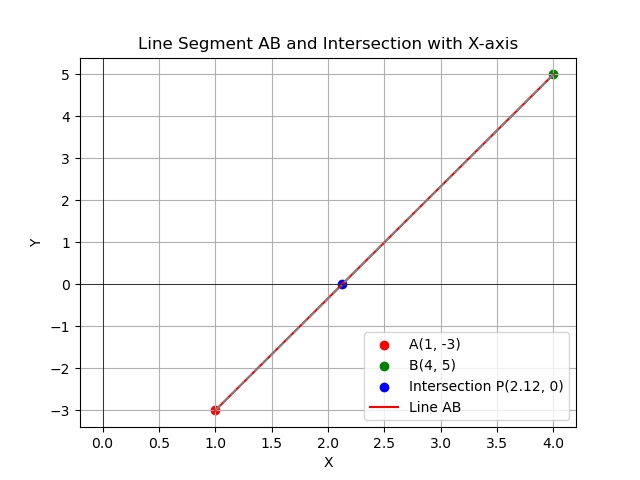
\includegraphics[width=\columnwidth]{figs/Figure_1.png}
    \caption{plot for line}
 \end{figure}
\end{frame}

\subsection{C Code}
\begin{frame}
\frametitle{C Code}
\begin{figure}[h]
    \centering
    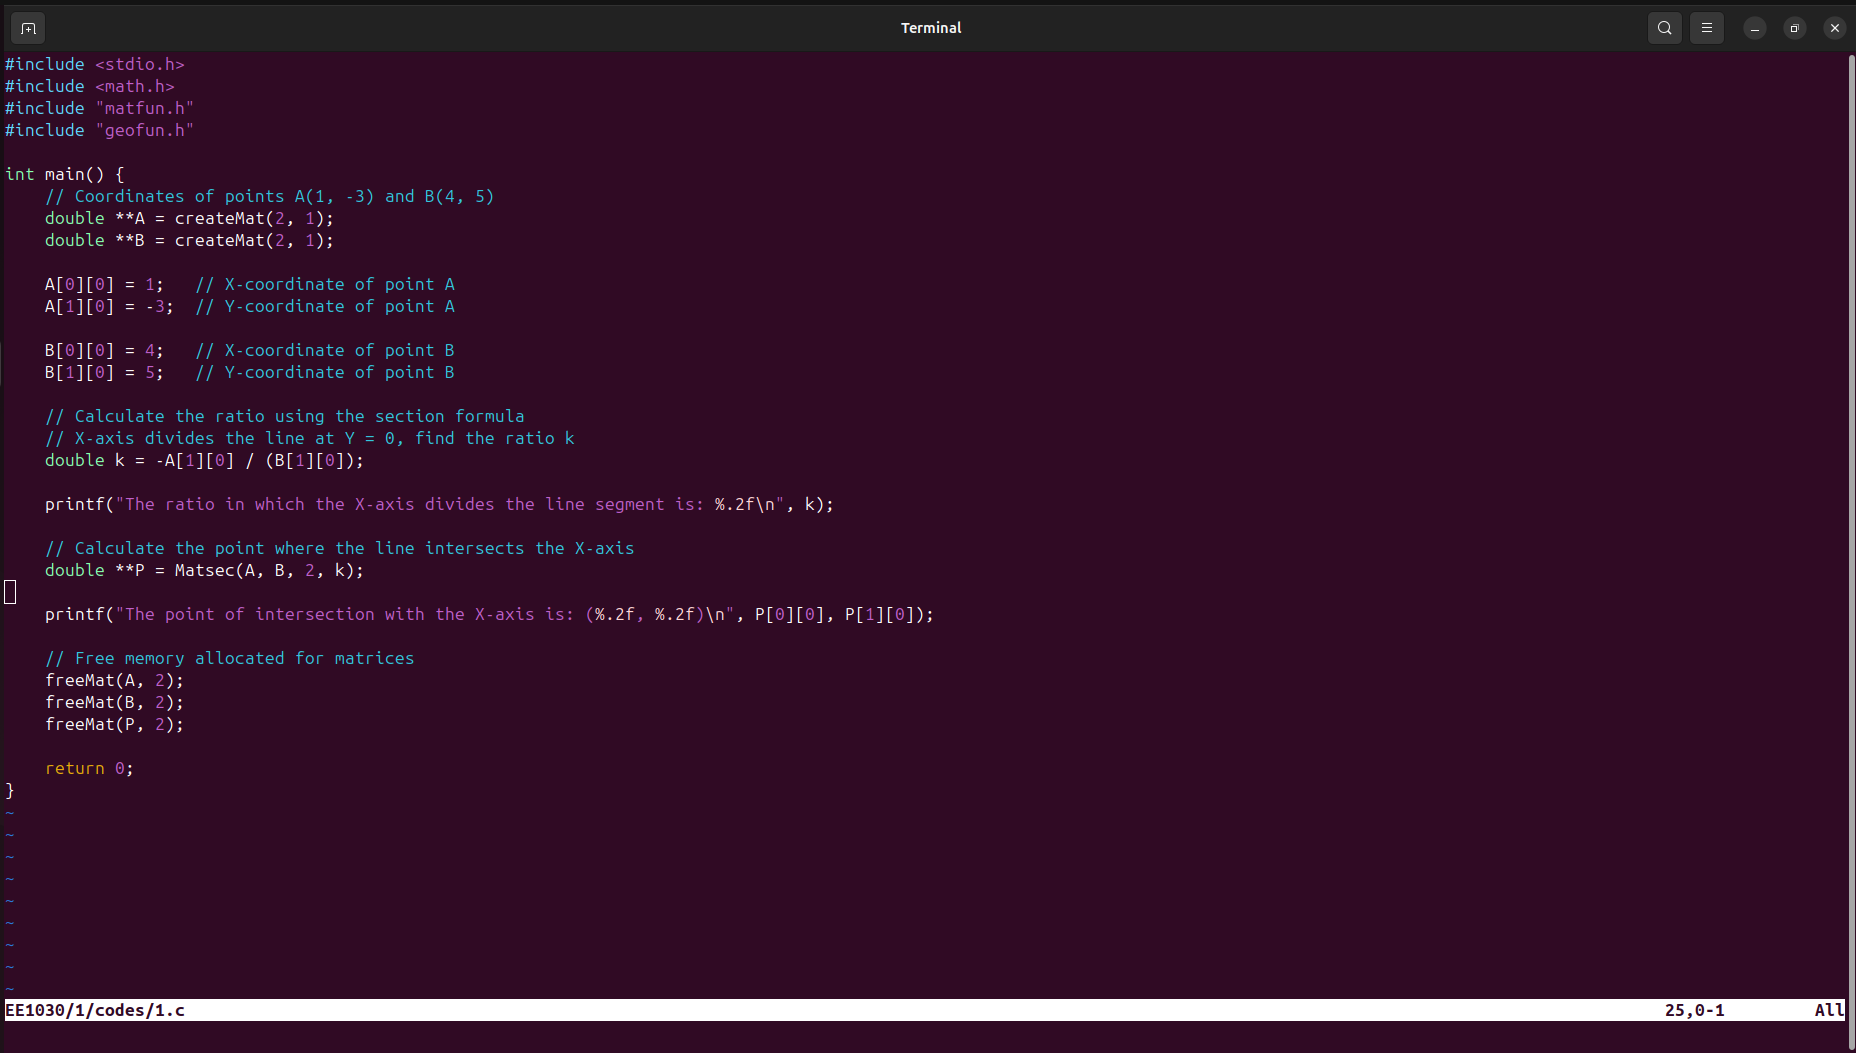
\includegraphics[width=\columnwidth]{figs/1.png}
 \end{figure}    
 \end{frame}
  \subsection{Python Code}
 \begin{frame}
\frametitle{Python Code}
\begin{figure}[h]
    \centering
    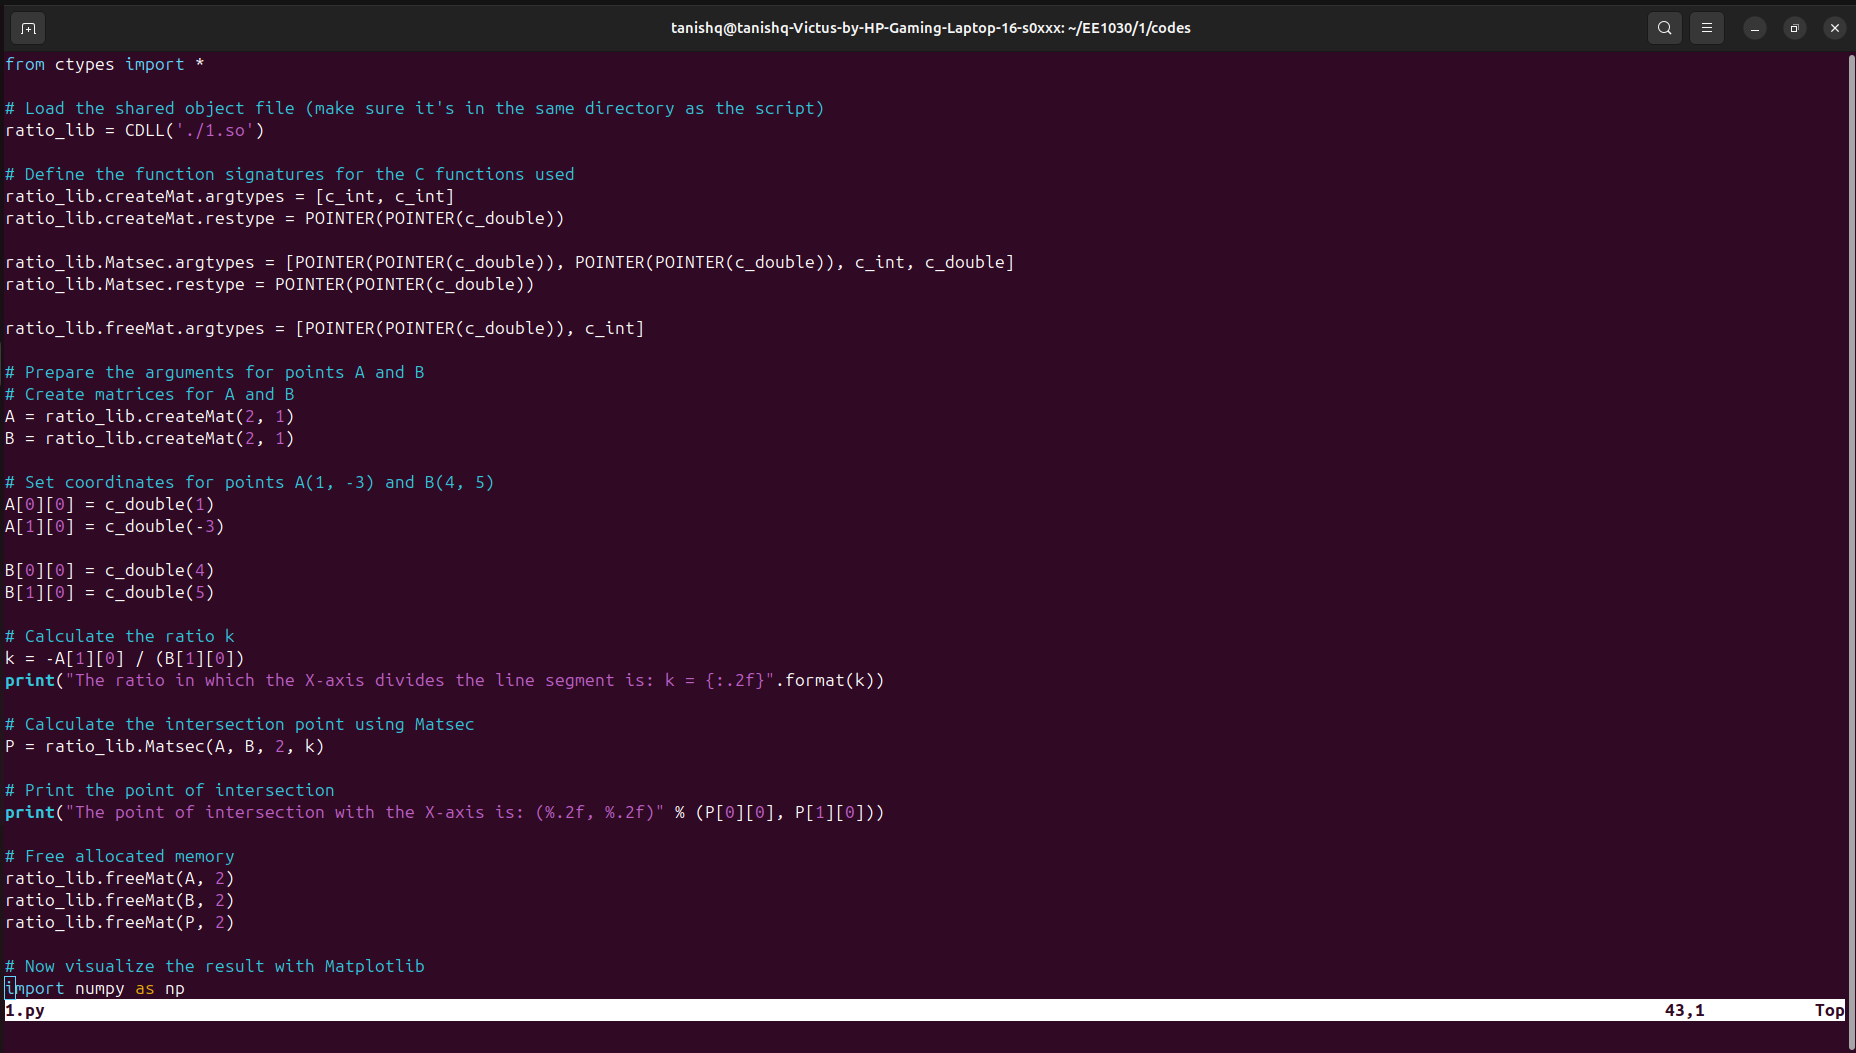
\includegraphics[width=\columnwidth]{figs/p1.png}
 \end{figure}    
 \end{frame}

 \subsection{Python Code}
 \begin{frame}
\frametitle{Python Code}
\begin{figure}[h]
    \centering
    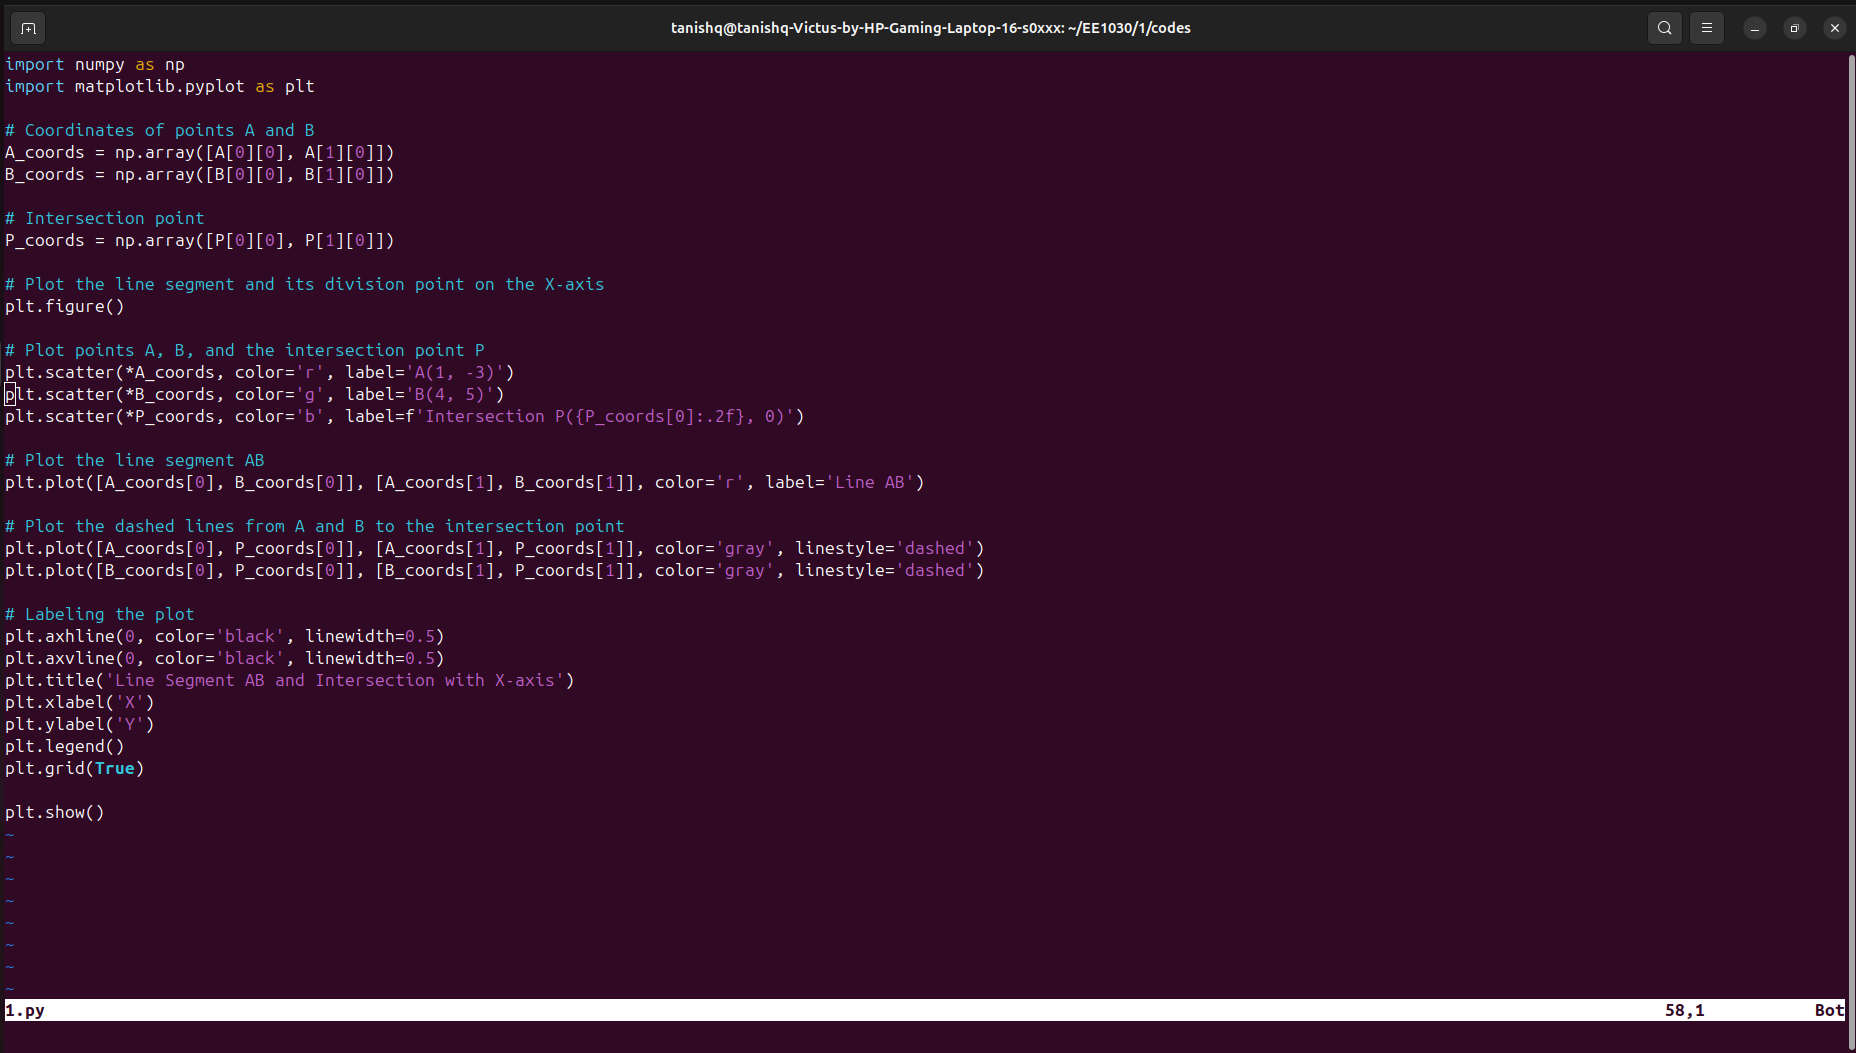
\includegraphics[width=\columnwidth]{figs/p2.png}
 \end{figure}    
 \end{frame}


\end{document}

